\documentclass[doc]{apa6}
\usepackage{lmodern}
\usepackage{amssymb,amsmath}
\usepackage{ifxetex,ifluatex}
\usepackage{fixltx2e} % provides \textsubscript
\ifnum 0\ifxetex 1\fi\ifluatex 1\fi=0 % if pdftex
  \usepackage[T1]{fontenc}
  \usepackage[utf8]{inputenc}
\else % if luatex or xelatex
  \ifxetex
    \usepackage{mathspec}
  \else
    \usepackage{fontspec}
  \fi
  \defaultfontfeatures{Ligatures=TeX,Scale=MatchLowercase}
\fi
% use upquote if available, for straight quotes in verbatim environments
\IfFileExists{upquote.sty}{\usepackage{upquote}}{}
% use microtype if available
\IfFileExists{microtype.sty}{%
\usepackage{microtype}
\UseMicrotypeSet[protrusion]{basicmath} % disable protrusion for tt fonts
}{}
\usepackage{hyperref}
\hypersetup{unicode=true,
            pdftitle={Working with list-columns in data.table},
            pdfauthor={Tyson S. Barrett},
            pdfkeywords={data.table, dplyr, list-columns, nesting},
            pdfborder={0 0 0},
            breaklinks=true}
\urlstyle{same}  % don't use monospace font for urls
\usepackage{color}
\usepackage{fancyvrb}
\newcommand{\VerbBar}{|}
\newcommand{\VERB}{\Verb[commandchars=\\\{\}]}
\DefineVerbatimEnvironment{Highlighting}{Verbatim}{commandchars=\\\{\}}
% Add ',fontsize=\small' for more characters per line
\usepackage{framed}
\definecolor{shadecolor}{RGB}{248,248,248}
\newenvironment{Shaded}{\begin{snugshade}}{\end{snugshade}}
\newcommand{\AlertTok}[1]{\textcolor[rgb]{0.94,0.16,0.16}{#1}}
\newcommand{\AnnotationTok}[1]{\textcolor[rgb]{0.56,0.35,0.01}{\textbf{\textit{#1}}}}
\newcommand{\AttributeTok}[1]{\textcolor[rgb]{0.77,0.63,0.00}{#1}}
\newcommand{\BaseNTok}[1]{\textcolor[rgb]{0.00,0.00,0.81}{#1}}
\newcommand{\BuiltInTok}[1]{#1}
\newcommand{\CharTok}[1]{\textcolor[rgb]{0.31,0.60,0.02}{#1}}
\newcommand{\CommentTok}[1]{\textcolor[rgb]{0.56,0.35,0.01}{\textit{#1}}}
\newcommand{\CommentVarTok}[1]{\textcolor[rgb]{0.56,0.35,0.01}{\textbf{\textit{#1}}}}
\newcommand{\ConstantTok}[1]{\textcolor[rgb]{0.00,0.00,0.00}{#1}}
\newcommand{\ControlFlowTok}[1]{\textcolor[rgb]{0.13,0.29,0.53}{\textbf{#1}}}
\newcommand{\DataTypeTok}[1]{\textcolor[rgb]{0.13,0.29,0.53}{#1}}
\newcommand{\DecValTok}[1]{\textcolor[rgb]{0.00,0.00,0.81}{#1}}
\newcommand{\DocumentationTok}[1]{\textcolor[rgb]{0.56,0.35,0.01}{\textbf{\textit{#1}}}}
\newcommand{\ErrorTok}[1]{\textcolor[rgb]{0.64,0.00,0.00}{\textbf{#1}}}
\newcommand{\ExtensionTok}[1]{#1}
\newcommand{\FloatTok}[1]{\textcolor[rgb]{0.00,0.00,0.81}{#1}}
\newcommand{\FunctionTok}[1]{\textcolor[rgb]{0.00,0.00,0.00}{#1}}
\newcommand{\ImportTok}[1]{#1}
\newcommand{\InformationTok}[1]{\textcolor[rgb]{0.56,0.35,0.01}{\textbf{\textit{#1}}}}
\newcommand{\KeywordTok}[1]{\textcolor[rgb]{0.13,0.29,0.53}{\textbf{#1}}}
\newcommand{\NormalTok}[1]{#1}
\newcommand{\OperatorTok}[1]{\textcolor[rgb]{0.81,0.36,0.00}{\textbf{#1}}}
\newcommand{\OtherTok}[1]{\textcolor[rgb]{0.56,0.35,0.01}{#1}}
\newcommand{\PreprocessorTok}[1]{\textcolor[rgb]{0.56,0.35,0.01}{\textit{#1}}}
\newcommand{\RegionMarkerTok}[1]{#1}
\newcommand{\SpecialCharTok}[1]{\textcolor[rgb]{0.00,0.00,0.00}{#1}}
\newcommand{\SpecialStringTok}[1]{\textcolor[rgb]{0.31,0.60,0.02}{#1}}
\newcommand{\StringTok}[1]{\textcolor[rgb]{0.31,0.60,0.02}{#1}}
\newcommand{\VariableTok}[1]{\textcolor[rgb]{0.00,0.00,0.00}{#1}}
\newcommand{\VerbatimStringTok}[1]{\textcolor[rgb]{0.31,0.60,0.02}{#1}}
\newcommand{\WarningTok}[1]{\textcolor[rgb]{0.56,0.35,0.01}{\textbf{\textit{#1}}}}
\usepackage{graphicx,grffile}
\makeatletter
\def\maxwidth{\ifdim\Gin@nat@width>\linewidth\linewidth\else\Gin@nat@width\fi}
\def\maxheight{\ifdim\Gin@nat@height>\textheight\textheight\else\Gin@nat@height\fi}
\makeatother
% Scale images if necessary, so that they will not overflow the page
% margins by default, and it is still possible to overwrite the defaults
% using explicit options in \includegraphics[width, height, ...]{}
\setkeys{Gin}{width=\maxwidth,height=\maxheight,keepaspectratio}
\IfFileExists{parskip.sty}{%
\usepackage{parskip}
}{% else
\setlength{\parindent}{0pt}
\setlength{\parskip}{6pt plus 2pt minus 1pt}
}
\setlength{\emergencystretch}{3em}  % prevent overfull lines
\providecommand{\tightlist}{%
  \setlength{\itemsep}{0pt}\setlength{\parskip}{0pt}}
\setcounter{secnumdepth}{0}
% Redefines (sub)paragraphs to behave more like sections
\ifx\paragraph\undefined\else
\let\oldparagraph\paragraph
\renewcommand{\paragraph}[1]{\oldparagraph{#1}\mbox{}}
\fi
\ifx\subparagraph\undefined\else
\let\oldsubparagraph\subparagraph
\renewcommand{\subparagraph}[1]{\oldsubparagraph{#1}\mbox{}}
\fi

%%% Use protect on footnotes to avoid problems with footnotes in titles
\let\rmarkdownfootnote\footnote%
\def\footnote{\protect\rmarkdownfootnote}


  \title{Working with list-columns in \texttt{data.table}}
    \author{Tyson S. Barrett\textsuperscript{1}}
    \date{}
  
\shorttitle{List-columns in data.table}
\affiliation{
\vspace{0.5cm}
\textsuperscript{1} Utah State University}
\keywords{data.table, dplyr, list-columns, nesting}
\usepackage{csquotes}
\usepackage{upgreek}
\captionsetup{font=singlespacing,justification=justified}

\usepackage{longtable}
\usepackage{lscape}
\usepackage{multirow}
\usepackage{tabularx}
\usepackage[flushleft]{threeparttable}
\usepackage{threeparttablex}

\newenvironment{lltable}{\begin{landscape}\begin{center}\begin{ThreePartTable}}{\end{ThreePartTable}\end{center}\end{landscape}}

\makeatletter
\newcommand\LastLTentrywidth{1em}
\newlength\longtablewidth
\setlength{\longtablewidth}{1in}
\newcommand{\getlongtablewidth}{\begingroup \ifcsname LT@\roman{LT@tables}\endcsname \global\longtablewidth=0pt \renewcommand{\LT@entry}[2]{\global\advance\longtablewidth by ##2\relax\gdef\LastLTentrywidth{##2}}\@nameuse{LT@\roman{LT@tables}} \fi \endgroup}

\authornote{

Correspondence concerning this article should be addressed to Tyson S. Barrett, 2800 Old Main, Logan, UT 84322. E-mail: \href{mailto:tyson.barrett@usu.edu}{\nolinkurl{tyson.barrett@usu.edu}}}

\abstract{
The use of \emph{list-columns} in data frames and tibbles is well documented (e.g.~Bryan, 2018), providing a cognitively efficient way to organize results of complex data (e.g.~several statistical models, groupings of text, data summaries, or even graphics) with corresponding data. For example, we can store text of a verse in a list for each verse, chapter, book, and volume. This allows the text to be of variable sizes without overly complicating or adding redundancies to the structure of the data. In turn, this can reduce the difficulty to appropriately analyze the data stored in the list-column. Because of its efficiency and speed, being able to use \texttt{data.table} to work with list-columns would be beneficial in many data contexts (i.e.~to reduce memory usage in large data sets). I show how one can create list-columns in a data table using \texttt{purrr::map()} and the \texttt{by} argument in \texttt{data.table}. I further show the \texttt{dplyr::group\_nest()} function and show a more efficient approach when using a data table. Results using \texttt{bench::mark()} show the speed and efficiency of using \texttt{data.table} to work with list-columns. An example walk-through is provided in the appendix herein.


}

\begin{document}
\maketitle

\hypertarget{introduction}{%
\section{Introduction}\label{introduction}}

The use of \emph{list-columns} in data frames and tibbles provides a cognitively efficient way to organize results of complex data (e.g.~several statistical models, groupings of text, data summaries, or even graphics) with corresponding data. It is often called \enquote{nested} data, where information is, in essence, nested within a column of data. For example, we can store text of a verse in a list for each verse, chapter, book, and volume. This allows the text to be of variable sizes without overly complicating or adding redundancies to the structure of the data. We could also nest students within classrooms, players within teams, and measures within individuals.

In turn, nesting can reduce the difficulty to appropriately analyze the data stored in the list-column. Using functions like \texttt{lapply()} or \texttt{purrr::map*()} makes further analysis of the nested data more intuitive.

Because of its efficiency and speed, being able to use \texttt{data.table} to work with list-columns would be beneficial in many data contexts (i.e.~to reduce memory usage in large data sets). Herein, I show how one can create list-columns in a data table using \texttt{purrr::map()} and the \texttt{by} argument in \texttt{data.table}. I further highlight the \texttt{dplyr::group\_nest()} function and show a more efficient approach when using a data table. Results using \texttt{bench::mark()} show the speed and efficiency of using \texttt{data.table} to work with list-columns.

This tutorial relies on several powerful packages, including \texttt{data.table}, \texttt{dplyr}, \texttt{bench}, \texttt{tidyr}, \texttt{papaja}, \texttt{stringr}, \texttt{ggplot2}, \texttt{ggbeeswarm}, \texttt{performance}, and \texttt{rvest} (Aust \& Barth, 2018; Clarke \& Sherrill-Mix, 2017; Dowle \& Srinivasan, 2019; Hester, 2019; Lüdecke, Makowski, \& Waggoner, 2019; Wickham, 2016, 2019b, 2019a; Wickham et al., 2019; Wickham \& Henry, 2019).

\hypertarget{example-with-nba-data}{%
\section{Example with NBA Data}\label{example-with-nba-data}}

\hypertarget{the-data}{%
\subsection{The Data}\label{the-data}}

To demonstrate the use of \emph{list-columns} in \texttt{data.table}, data from \href{nbastuffer.com}{NBA Stuffer} will be scraped to get information on players from the 2017-2018 and 2018-2019 seasons. First, the HTML data are read in, the tables with player data by year are then extracted using a custom function, indicators are added, and then combined into a single data table for the player data.

\begin{Shaded}
\begin{Highlighting}[]
\NormalTok{url_}\DecValTok{2018}\NormalTok{ <-}\StringTok{ "https://www.nbastuffer.com/2017-2018-nba-player-stats/"}
\NormalTok{url_}\DecValTok{2019}\NormalTok{ <-}\StringTok{ "https://www.nbastuffer.com/2018-2019-nba-player-stats/"}
\NormalTok{players_}\DecValTok{2018}\NormalTok{ <-}\StringTok{ }\KeywordTok{read_html}\NormalTok{(url_}\DecValTok{2018}\NormalTok{)}
\NormalTok{players_}\DecValTok{2019}\NormalTok{ <-}\StringTok{ }\KeywordTok{read_html}\NormalTok{(url_}\DecValTok{2019}\NormalTok{)}

\NormalTok{extract_fun <-}\StringTok{ }\ControlFlowTok{function}\NormalTok{(html)\{}
  \KeywordTok{html_nodes}\NormalTok{(html, }\StringTok{"table"}\NormalTok{) }\OperatorTok\StringTok{ }
\StringTok{    }\NormalTok{.[}\DecValTok{2}\NormalTok{] }\OperatorTok\StringTok{ }
\StringTok{    }\KeywordTok{html_table}\NormalTok{(}\DataTypeTok{fill =} \OtherTok{TRUE}\NormalTok{) }\OperatorTok\StringTok{ }
\StringTok{    }\NormalTok{.[[}\DecValTok{1}\NormalTok{]] }
\NormalTok{\}}

\NormalTok{player_}\DecValTok{2018}\NormalTok{ <-}\StringTok{ }
\StringTok{  }\KeywordTok{extract_fun}\NormalTok{(players_}\DecValTok{2018}\NormalTok{) }\OperatorTok\StringTok{ }
\StringTok{  }\KeywordTok{mutate}\NormalTok{(}\DataTypeTok{year =} \DecValTok{2018}\NormalTok{,}
         \DataTypeTok{AGE =} \KeywordTok{as.numeric}\NormalTok{(AGE))}
\NormalTok{player_}\DecValTok{2019}\NormalTok{ <-}\StringTok{ }
\StringTok{  }\KeywordTok{extract_fun}\NormalTok{(players_}\DecValTok{2019}\NormalTok{) }\OperatorTok\StringTok{ }
\StringTok{  }\KeywordTok{mutate}\NormalTok{(}\DataTypeTok{year =} \DecValTok{2019}\NormalTok{)}
\NormalTok{players <-}\StringTok{ }
\StringTok{  }\KeywordTok{bind_rows}\NormalTok{(player_}\DecValTok{2018}\NormalTok{, player_}\DecValTok{2019}\NormalTok{) }\OperatorTok\StringTok{ }
\StringTok{  }\KeywordTok{clean_names}\NormalTok{() }\OperatorTok\StringTok{ }
\StringTok{  }\KeywordTok{rename}\NormalTok{(}\DataTypeTok{ppg =}\NormalTok{ ppg_points_points_per_game,}
         \DataTypeTok{apg =}\NormalTok{ apg_assists_assists_per_game) }\OperatorTok\StringTok{ }
\StringTok{  }\KeywordTok{data.table}\NormalTok{()}
\end{Highlighting}
\end{Shaded}

Below is a subset of this data set.

\begin{verbatim}
##         full_name  mpg  ppg apg
## 1:   Aaron Brooks  5.9  2.3 0.6
## 2:   Aaron Gordon 32.9 17.6 2.3
## 3: Aaron Harrison 25.9  6.7 1.2
## 4:  Aaron Jackson 34.5  8.0 1.0
## 5:    Abdel Nader 10.9  3.0 0.5
## 6:  Adreian Payne  8.5  4.2 0.0
\end{verbatim}

\hypertarget{nesting-players-within-teams}{%
\subsection{Nesting Players within Teams}\label{nesting-players-within-teams}}

In \texttt{dplyr} the \texttt{group\_nest()} function is valuable when creating list-columns based on a grouping variable. It takes the data by group and puts it all in a list-column. Figure \ref{process} highlights the process of taking a data frame and creating a nested data frame with a list-column. That is, all data from variables \texttt{x}, \texttt{y}, and \texttt{z} relating to each group is split into a distinct data frame and stored within the \texttt{data} column.

\begin{figure}[htb]
  \centering
  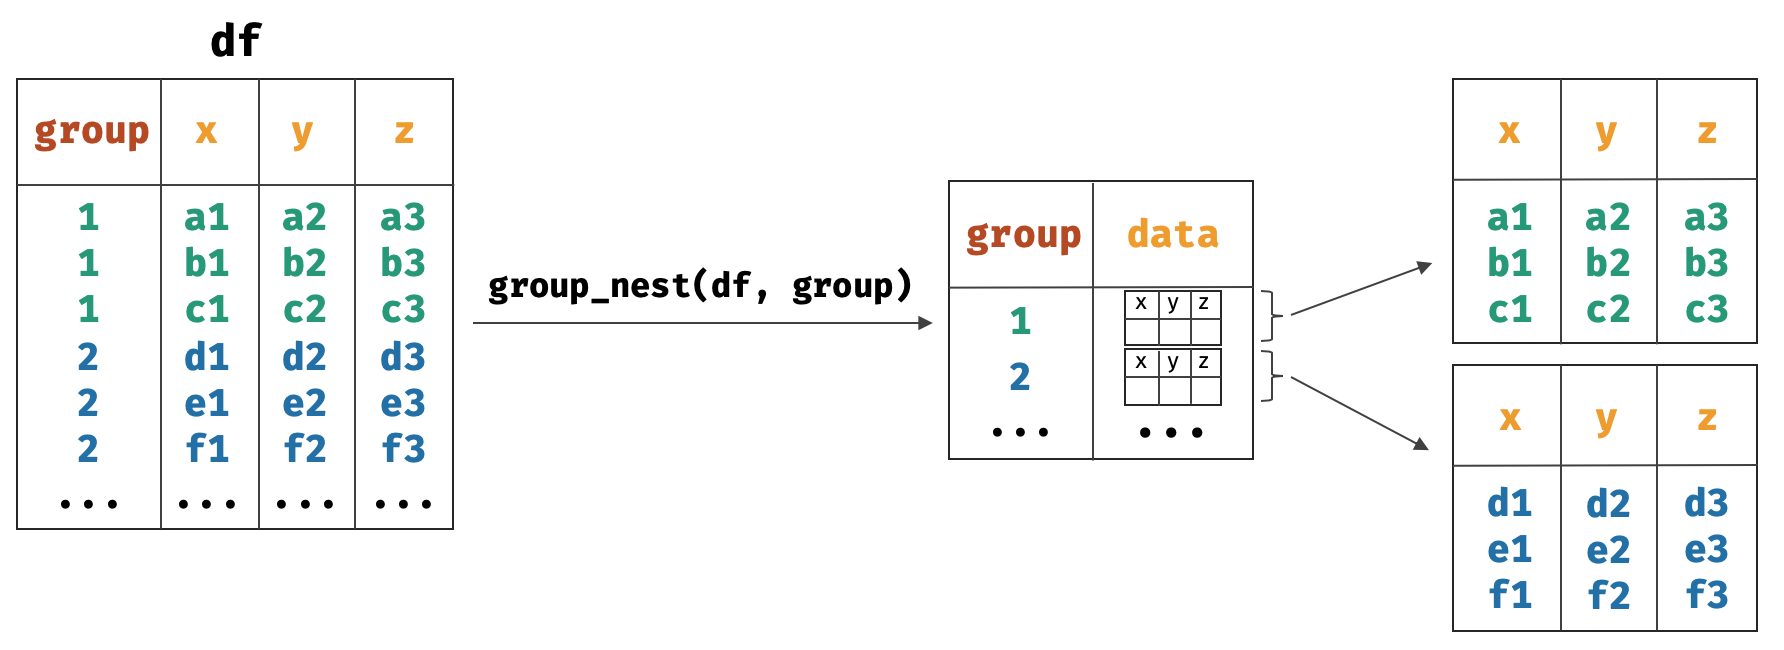
\includegraphics[width=\textwidth]{fig_process.png}
  \caption{Speed comparisons for each nesting approach.}
  \label{process}
\end{figure}

Overall, this function is efficient and fast but by using \texttt{data.table} it can be faster. This will be shown using the following function:

\begin{Shaded}
\begin{Highlighting}[]
\NormalTok{group_nest_dt <-}\StringTok{ }\ControlFlowTok{function}\NormalTok{(dt, ..., }\DataTypeTok{.key =} \StringTok{"data"}\NormalTok{)\{}
  \KeywordTok{stopifnot}\NormalTok{(}\KeywordTok{is.data.table}\NormalTok{(dt))}

\NormalTok{  by <-}\StringTok{ }\KeywordTok{substitute}\NormalTok{(}\KeywordTok{list}\NormalTok{(...))}
  
\NormalTok{  express <-}\StringTok{ }\NormalTok{dt[, }\KeywordTok{list}\NormalTok{(}\KeywordTok{list}\NormalTok{(.SD)), by =}\StringTok{ }\KeywordTok{eval}\NormalTok{(by)]}
  \KeywordTok{setnames}\NormalTok{(express, }\DataTypeTok{old =} \StringTok{"V1"}\NormalTok{, }\DataTypeTok{new =}\NormalTok{ .key)}
\NormalTok{  express}
\NormalTok{\}}
\end{Highlighting}
\end{Shaded}

In essence, this function takes a data table, then creates a list of the data table per group specified in the \texttt{by} argument.

\begin{Shaded}
\begin{Highlighting}[]
\KeywordTok{group_nest_dt}\NormalTok{(players, team) }\OperatorTok\StringTok{ }
\StringTok{  }\KeywordTok{head}\NormalTok{()}
\end{Highlighting}
\end{Shaded}

\begin{verbatim}
##    team         data
## 1:  Min <data.table>
## 2:  Orl <data.table>
## 3:  Dal <data.table>
## 4:  Hou <data.table>
## 5:  Bos <data.table>
## 6:  Ind <data.table>
\end{verbatim}

This is nearly identical to the \texttt{dplyr::group\_nest()} function, in terms of output, but has data tables in the list-column instead of tibbles.

\begin{Shaded}
\begin{Highlighting}[]
\KeywordTok{group_nest}\NormalTok{(players, team) }\OperatorTok\StringTok{ }
\StringTok{  }\KeywordTok{head}\NormalTok{()}
\end{Highlighting}
\end{Shaded}

\begin{verbatim}
## # A tibble: 6 x 2
##   team  data              
##   <chr> <list>            
## 1 Atl   <tibble [44 x 30]>
## 2 Bos   <tibble [37 x 30]>
## 3 Bro   <tibble [41 x 30]>
## 4 Cha   <tibble [34 x 30]>
## 5 Chi   <tibble [43 x 30]>
## 6 Cle   <tibble [49 x 30]>
\end{verbatim}

Importantly, Figure \ref{speed} presents the timings from \texttt{bench::mark()} across the two approaches, showing \texttt{group\_nest\_dt()} is somewhat faster. The memory allocated is very similar, with \texttt{group\_nest\_dt()} allocating 451KB and \texttt{group\_nest()} allocating 335KB.

\begin{figure}[htb]
  \centering
  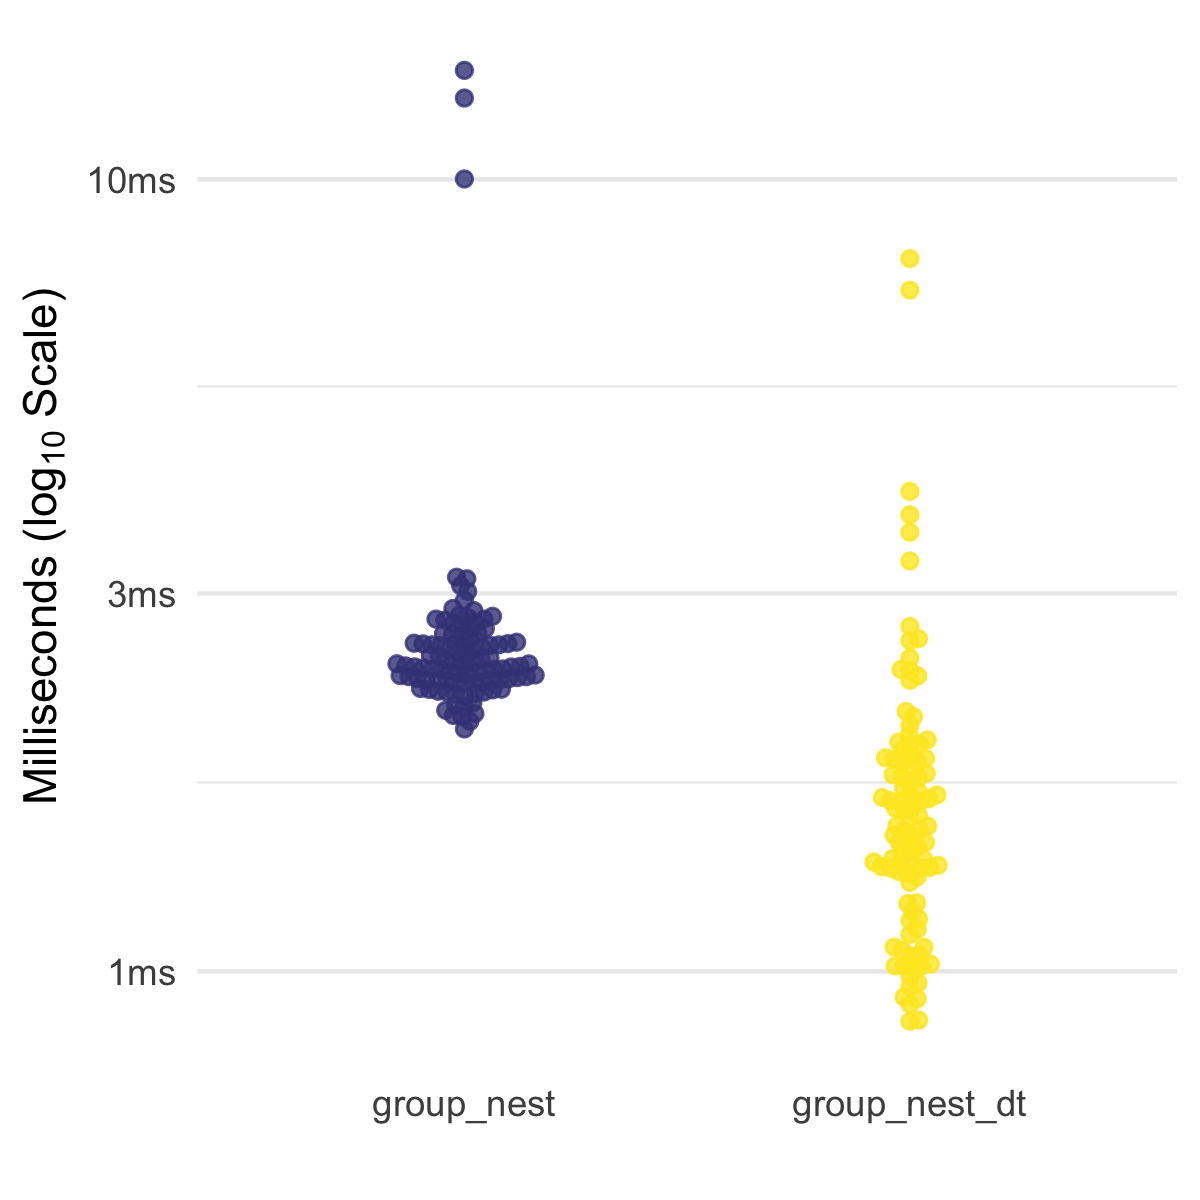
\includegraphics[width=0.6\textwidth]{timings_manuscript.png}
  \caption{Speed comparisons for each nesting approach.}
  \label{speed}
\end{figure}

This nesting approach can be used with multiple grouping variables too. For example, we can nest by both \texttt{team} and \texttt{year}, as is done below.

\begin{Shaded}
\begin{Highlighting}[]
\KeywordTok{group_nest_dt}\NormalTok{(players, team, year) }\OperatorTok\StringTok{ }
\StringTok{  }\KeywordTok{head}\NormalTok{()}
\end{Highlighting}
\end{Shaded}

\begin{verbatim}
##    team year         data
## 1:  Min 2018 <data.table>
## 2:  Orl 2018 <data.table>
## 3:  Dal 2018 <data.table>
## 4:  Hou 2018 <data.table>
## 5:  Bos 2018 <data.table>
## 6:  Ind 2018 <data.table>
\end{verbatim}

\hypertarget{modeling-within-the-nest}{%
\subsection{Modeling within the Nest}\label{modeling-within-the-nest}}

Often, the nested data can provide an intuitive format to run several models to understand key features of the data within the groups. Below, the relationship between points-per-game and assists-per-game for each team and year is modeled and then the \(R^2\) of the models are extracted.

\begin{Shaded}
\begin{Highlighting}[]
\NormalTok{players_nested <-}\StringTok{ }\KeywordTok{group_nest_dt}\NormalTok{(players, team, year) }\OperatorTok\StringTok{ }
\StringTok{  }\NormalTok{.[, ppg_apg    }\OperatorTok{:}\ErrorTok{=}\StringTok{ }\NormalTok{purrr}\OperatorTok{::}\KeywordTok{map}\NormalTok{(data, }\OperatorTok{~}\KeywordTok{lm}\NormalTok{(ppg }\OperatorTok{~}\StringTok{ }\NormalTok{apg, }\DataTypeTok{data =}\NormalTok{ .x))] }\OperatorTok\StringTok{ }
\StringTok{  }\NormalTok{.[, r2_list    }\OperatorTok{:}\ErrorTok{=}\StringTok{ }\NormalTok{purrr}\OperatorTok{::}\KeywordTok{map}\NormalTok{(ppg_apg, }\OperatorTok{~}\NormalTok{performance}\OperatorTok{::}\KeywordTok{r2}\NormalTok{(.x))] }\OperatorTok\StringTok{ }
\StringTok{  }\NormalTok{.[, r2_ppg_apg }\OperatorTok{:}\ErrorTok{=}\StringTok{ }\NormalTok{purrr}\OperatorTok{::}\KeywordTok{map_dbl}\NormalTok{(r2_list, }\OperatorTok{~}\NormalTok{.x[[}\DecValTok{1}\NormalTok{]])]}
\KeywordTok{head}\NormalTok{(players_nested)}
\end{Highlighting}
\end{Shaded}

\begin{verbatim}
##    team year         data ppg_apg      r2_list r2_ppg_apg
## 1:  Min 2018 <data.table>    <lm> <r2_generic>  0.4662060
## 2:  Orl 2018 <data.table>    <lm> <r2_generic>  0.4357684
## 3:  Dal 2018 <data.table>    <lm> <r2_generic>  0.4305347
## 4:  Hou 2018 <data.table>    <lm> <r2_generic>  0.6967150
## 5:  Bos 2018 <data.table>    <lm> <r2_generic>  0.6043402
## 6:  Ind 2018 <data.table>    <lm> <r2_generic>  0.6060465
\end{verbatim}

\noindent This produces two list-columns (\texttt{ppg\_apg} and \texttt{r2\_list}) and a numeric vector (\texttt{r2\_ppg\_apg}) all organized by team and year. This information is then readily available to plot. For example, we can look at the change in how related points-per-game and assists-per-game are by team and year.

\begin{Shaded}
\begin{Highlighting}[]
\KeywordTok{library}\NormalTok{(ggrepel)}
\KeywordTok{theme_set}\NormalTok{(}\KeywordTok{theme_minimal}\NormalTok{() }\OperatorTok{+}
\StringTok{          }\KeywordTok{theme}\NormalTok{(}\DataTypeTok{panel.grid.major.x =} \KeywordTok{element_blank}\NormalTok{(),}
                \DataTypeTok{legend.position =} \StringTok{"none"}\NormalTok{))}

\NormalTok{ex_fig <-}\StringTok{ }\NormalTok{players_nested }\OperatorTok\StringTok{ }
\StringTok{  }\KeywordTok{dcast}\NormalTok{(team }\OperatorTok{~}\StringTok{ }\NormalTok{year, }\DataTypeTok{value.var =} \StringTok{"r2_ppg_apg"}\NormalTok{) }\OperatorTok\StringTok{ }
\StringTok{  }\KeywordTok{ggplot}\NormalTok{(}\KeywordTok{aes}\NormalTok{(}\StringTok{`}\DataTypeTok{2018}\StringTok{`}\NormalTok{, }\StringTok{`}\DataTypeTok{2019}\StringTok{`}\NormalTok{, }\DataTypeTok{group =}\NormalTok{ team)) }\OperatorTok{+}
\StringTok{    }\KeywordTok{geom_point}\NormalTok{() }\OperatorTok{+}
\StringTok{    }\KeywordTok{geom_text_repel}\NormalTok{(}\KeywordTok{aes}\NormalTok{(}\DataTypeTok{label =}\NormalTok{ team)) }\OperatorTok{+}
\StringTok{    }\KeywordTok{geom_abline}\NormalTok{(}\DataTypeTok{slope =} \DecValTok{1}\NormalTok{) }\OperatorTok{+}
\StringTok{    }\KeywordTok{coord_fixed}\NormalTok{(}\DataTypeTok{ylim =} \KeywordTok{c}\NormalTok{(}\DecValTok{0}\NormalTok{,}\DecValTok{1}\NormalTok{),}
                \DataTypeTok{xlim =} \KeywordTok{c}\NormalTok{(}\DecValTok{0}\NormalTok{,}\DecValTok{1}\NormalTok{))}
\end{Highlighting}
\end{Shaded}

\begin{figure}[htb]
  \centering
  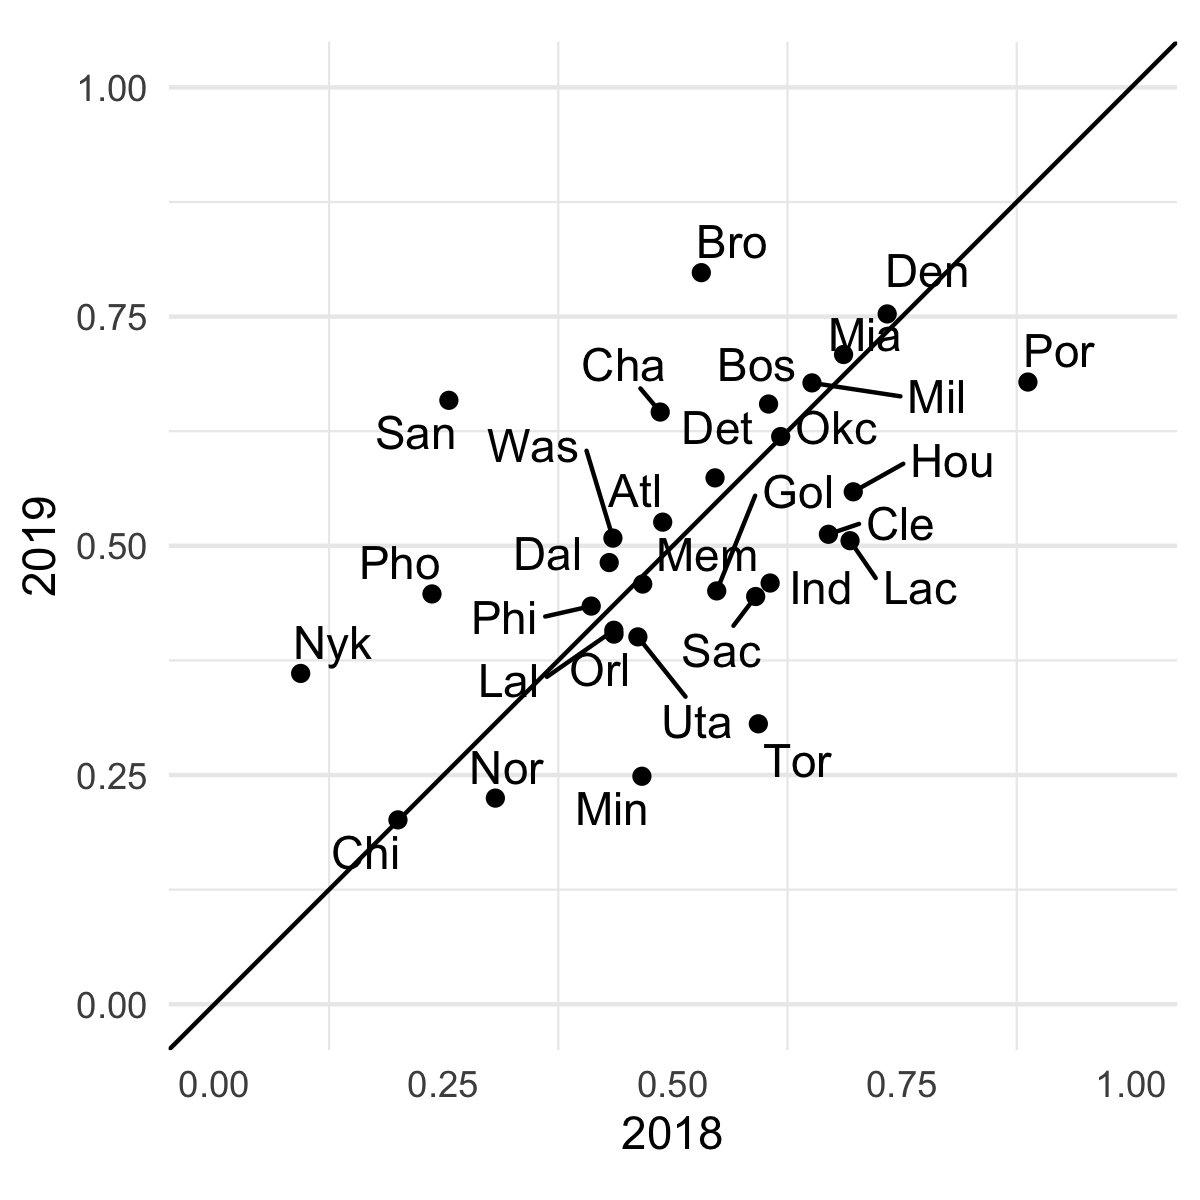
\includegraphics[width=0.6\textwidth]{ex_fig.png}
  \caption{Speed comparisons for each nesting approach.}
  \label{speed}
\end{figure}

\hypertarget{discussion}{%
\section{Discussion}\label{discussion}}

List-columns are a useful approach to organizing

\hypertarget{references}{%
\section{References}\label{references}}

\begingroup
\setlength{\parindent}{-0.5in}
\setlength{\leftskip}{0.5in}

\hypertarget{refs}{}
\leavevmode\hypertarget{ref-R-papaja}{}%
Aust, F., \& Barth, M. (2018). \emph{papaja: Create APA manuscripts with R Markdown}. Retrieved from \url{https://github.com/crsh/papaja}

\leavevmode\hypertarget{ref-jenny}{}%
Bryan, J. (2018). List columns (as part of "purrr tutorial"). Retrieved from \url{https://jennybc.github.io/purrr-tutorial/ls13_list-columns.html}

\leavevmode\hypertarget{ref-R-ggbeeswarm}{}%
Clarke, E., \& Sherrill-Mix, S. (2017). \emph{Ggbeeswarm: Categorical scatter (violin point) plots}. Retrieved from \url{https://github.com/eclarke/ggbeeswarm}

\leavevmode\hypertarget{ref-R-data.table}{}%
Dowle, M., \& Srinivasan, A. (2019). \emph{Data.table: Extension of `data.frame`}. Retrieved from \url{https://CRAN.R-project.org/package=data.table}

\leavevmode\hypertarget{ref-R-bench}{}%
Hester, J. (2019). \emph{Bench: High precision timing of r expressions}. Retrieved from \url{https://CRAN.R-project.org/package=bench}

\leavevmode\hypertarget{ref-R-performance}{}%
Lüdecke, D., Makowski, D., \& Waggoner, P. (2019). \emph{Performance: Assessment of regression models performance}. Retrieved from \url{https://easystats.github.io/performance/}

\leavevmode\hypertarget{ref-R-ggplot2}{}%
Wickham, H. (2016). \emph{Ggplot2: Elegant graphics for data analysis}. Springer-Verlag New York. Retrieved from \url{https://ggplot2.tidyverse.org}

\leavevmode\hypertarget{ref-R-rvest}{}%
Wickham, H. (2019a). \emph{Rvest: Easily harvest (scrape) web pages}. Retrieved from \url{https://CRAN.R-project.org/package=rvest}

\leavevmode\hypertarget{ref-R-stringr}{}%
Wickham, H. (2019b). \emph{Stringr: Simple, consistent wrappers for common string operations}. Retrieved from \url{https://CRAN.R-project.org/package=stringr}

\leavevmode\hypertarget{ref-R-dplyr}{}%
Wickham, H., François, R., Henry, L., \& Müller, K. (2019). \emph{Dplyr: A grammar of data manipulation}. Retrieved from \url{https://CRAN.R-project.org/package=dplyr}

\leavevmode\hypertarget{ref-R-tidyr}{}%
Wickham, H., \& Henry, L. (2019). \emph{Tidyr: Easily tidy data with 'spread()' and 'gather()' functions}. Retrieved from \url{https://CRAN.R-project.org/package=tidyr}

\endgroup


\end{document}
